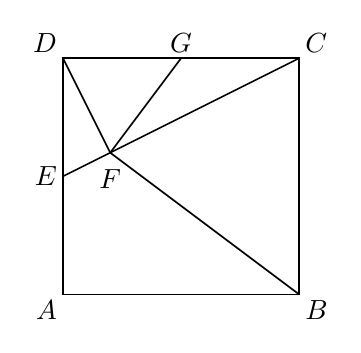
\begin{tikzpicture}[x=1cm,y=1cm,font=\normalsize,
 geometry edge/.style={solid,line width=.6pt},
 geometry mark/.style={solid,line width=.6pt},
 geometry label/.style={font=\normalsize,inner sep=2pt}]
\coordinate (D) at (0,0);
\coordinate (C) at (3,0);
\coordinate (G) at (1.5,0);
\coordinate (E) at (0,-1.5);
\coordinate (F) at (0.6,-1.2);
\coordinate (A) at (0,-3);
\coordinate (B) at (3,-3);
\draw[geometry edge] (A)--(B)--(C)--(D)--cycle;
\draw[geometry edge] (D)--(F)--(B);
\draw[geometry edge] (C)--(F)--(E);
\draw[geometry edge] (G)--(F);
\node[geometry label,above left] at (D) {$D$};
\node[geometry label,above] at (G) {$G$};
\node[geometry label,above right] at (C) {$C$};
\node[geometry label,left] at (E) {$E$};
\node[geometry label,below,yshift=-4pt] at (F) {$F$};
\node[geometry label,below left] at (A) {$A$};
\node[geometry label,below right] at (B) {$B$};
\end{tikzpicture}
